\chapter{НАУЧНАЯ СОСТАВЛЯЮЩАЯ}
\label{chap:research}
\aftertitle

В этой главе рассматривается экспериментальная работа по проверке разработанного сервиса и анализу новостей с его помощью. Описаны проведенные эксперименты по анализу новостей.

В исследовании использовались исторические данные новостей, собранные за 2020 год.

\section{Анализ количества новостей}

В первую очередь был произведен анализ количества новостей в день за исследуемый промежуток времени. На рисунке \ref{img:news-count} представлен график количества новостей за день. Минимальное количество новостей в день 165, максимальное ~-- 2890, а среднее ~--- 1907.

\begin{figure}[h]
    \centering
    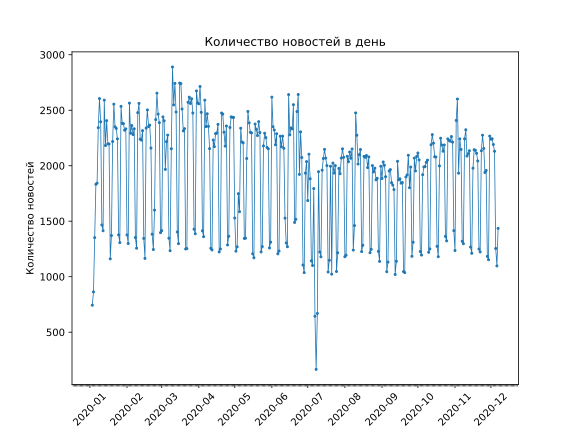
\includegraphics[width=\linewidth]{images/news-count.png}
    \caption{Количество новостей в день}
    \label{img:news-count}
\end{figure}

\section{Исследование расстояния между новостями}

Была изучена статистика попарного косинусного расстояния между векторным представлением новостей за день.

Косинусное расстояние двух векторов $a$ и $b$ ~-- это метрика схожести двух ненулевых векторов, определяемая как косинус угла между ними (\ref{eq:cosine-dist}).

\begin{equation}
    cos(\theta) = \frac{\vec{a} \cdot \vec{b}}{||\vec{a}|| \cdot ||{b}||}
    \label{eq:cosine-dist}
\end{equation}

Таким образом, эмбеддинги близких по смыслу новостей будут представлять собой два вектора с приблизительно одинаковым направлением, и их косинусное расстояние будет близко к единице. Наоборот, эмбеддинги противоположных по смыслу новостей будут представлять собой два вектора, направленные в противоположенные стороны, и их косинусное расстояние будет близко к минус единице. Таким образом, чем ближе косинусное расстояние к единице, тем более похожи новости.

Так как косинусное расстояние между векторным представлением соответствует семантической близости новостей друг другу, то статистика попарных расстояний может отражать характер распределения новостей по темам. Если за выбранный временной интервал много новостей на различные, то косинусное расстояние между ними будет близко к -1, и статистика попарных расстояния будут сдвинута в сторону меньших значений. Наоборот, если новости за выбранный временной интервал были на схожие темы, то косинусное расстояние будет близко к 1 , и статистика распределения попарных расстояний будет сдвинута в сторону больших значений.

На рисунке \ref{img:distances-distribution} показано сравнение распределения попарных косинусных расстояний за два дня. Распределение в области малых значений, т.е. новостей, которые не похожи друг на друга, совпадает. Различие наблюдается в области больших значений, т.е. новостей, которые похожи друг на друга. За один день наблюдается большее значение плотности распределения в области больших значений, чем за другой день, что говорит о том, что в этот день было больше новостей на близкие темы.

\begin{figure}[h]
    \centering
    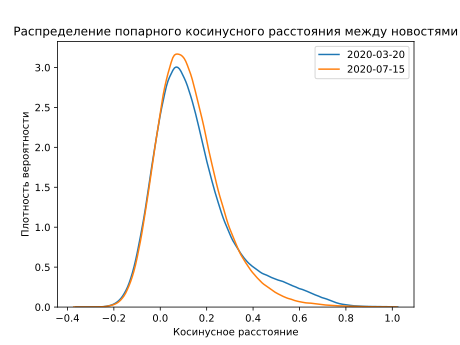
\includegraphics[width=\linewidth]{images/distances-distribution.png}
    \caption{Сравнение распределение косинусного расстояния между новостями за два дня}
    \label{img:distances-distribution}
\end{figure}

Так как построение распределения для всех дней не является наглядной визуализацией, то для изучения динамики изменения распределения попарных косинусных расстояний межу новостями, было решено построить графики отдельных квантилей: 50\% (медиана), 75\% и 90\%. График изменения распределения попарного косинусного расстояния по дням представлен на рисунке \ref{img:distances}.

\begin{figure}[h]
    \centering
    \includegraphics[width=\linewidth]{images/distances.png}
    \caption{Изменение распределения попарного косинусного расстояния по дням}
    \label{img:distances}
\end{figure}

На этом графике показаны значения трех квантилей: 50\% (синий), 75\% (оранжевый) и 90\% (зеленый) в виде точек. Каждая точка показывает значение соответствующего квантиля распределения попарного косинусного расстояния между новостями за один день. На графике мы  можем отчетливо видеть колебания с периодом 7 дней, по всей видимости, связанные с недельными изменениями в  распределении тематик новостей.

Значения 50\% квантиля практически не изменяются во времени, не считая недельных колебаний. Это согласуется с рассмотренным ранее на рисунке \ref{img:distances-distribution} сравнением распределения попарных косинусных расстояний между новостями за два дня, на котором видно, что в области малых значений распределение практически совпадает. Медианное значение 50\%-квантиля составляет 0.12, что соответствует непохожим новостям. Таким образом, распределение непохожих новостей мало меняется во времени, что может говорить о том, что в новостях всегда (за исключением недельных колебаний) охватывается примерно одинаково широкий круг тем.

Поведение значения 75\% квантиля мало отличается от поведения значений 50\% квантиля, но в них наблюдается небольшое увеличение в определенные моменты времени.

Наибольший интерес представляет поведение 90\% квантиля. Среди этих значений недельные колебания не так выражены, но выражен значительный рост значений в определенный период времени. Это говорит о том, что в этот момент времени распределение попарных косинусных расстояний между новостями было смещено в область больших значений, т.е. было больше новостей на похожие темы. По времени этот момент совпадает с началом пандемии коронавируса, карантина и экономического кризиса. Вероятно, эти темы обсуждались более активно, чем другие, что вызвало появление большего количества новостей на сходные тематики и смещение распределения попарного косинусного расстояния между новостями.

Таким образом, исследование распределения попарного косинусного расстояния между новостями может служить инструментом для выявления периодов с активным обсуждением тех или иных тем. При этом, наибольший интерес представляют больше квантили, такие как 90\%-квантиль.

